\chapter{Consuntivo}\label{chap:consuntivo}
In questa sezione del documento sono riportati i consuntivi orari ed economici di ogni sprint, frutto dell'effettivo grado di avanzamento di questo progetto.\\
A facilitare la lettura dei dati, le tabelle dei consuntivi orari ed economici sono accompagnate da grafici riportanti la distribuzione dei ruoli per membro in uno sprint e il budget rimanente in relazione al costo effettivo.\\ \\
Nel consuntivo orario, così come per i preventivi, i ruoli vengono riportati con le seguenti abbreviazioni:
\begin{itemize}
    \item R.: responsabile;
    \item Am.: amministratore;
    \item Pj.: progettista;
    \item An.: analista;
    \item Pg.: programmatore;
    \item V.: verificatore.
\end{itemize}
Ogni consuntivo di periodo è accompagnato da un'analisi retrospettiva elaborata durante una riunione interna di fine sprint, le cui considerazioni saranno riflesse in aggiornamenti della pianificazione, dei tempi e dei costi preventivati qualora necessario.
\newpage

\section{Requirements and Technology Baseline}
\subsection{Primo sprint: 2023/11/06 - 2023/11/19}
\subsubsection{Consuntivo orario}
{
\setlength{\tabcolsep}{10pt}
\renewcommand{\arraystretch}{1.5}
\rowcolors{2}{oddrow}{evenrow}
\begin{table}[h!]
    \centering
    \begin{tabularx}{\textwidth}{| l | c | c | c | c | c | c | X |}
        \hline
        \rowcolor{headerrow} \textbf{\textcolor{white}{Membro}} & \textbf{\textcolor{white}{R.}} & \textbf{\textcolor{white}{Am.}} & \textbf{\textcolor{white}{Pj.}} & \textbf{\textcolor{white}{An.}} & \textbf{\textcolor{white}{Pg.}} & \textbf{\textcolor{white}{V.}} & \textbf{\textcolor{white}{Totale}} \\
        \hline
        Andrea Cecchin & - & 1 & - & 8 & - & 1 & \textbf{10} \\
        \hline
        Marco Dolzan & - & 1 & - & 6 & - & 2 & \textbf{9} \\
        \hline
        Francesco Ferraioli & - & 9 & - & - & - & 1 & \textbf{10} \\
        \hline  
        Francesco Giacomuzzo & - & 1 & - & 2 & - & 4 & \textbf{7} \\
        \hline
        Leonardo Lago & - & 2 & - & 6 & - & 1 & \textbf{9} \\
        \hline
        Giovanni Menon & 7 & - & - & 1 & - & - & \textbf{8} \\
        \hline
        Anna Nordio & - & 2 & - & 2 & - & 5 & \textbf{9} \\
        \hline
    \cellcolor{headerrow} \textbf{\textcolor{white}{Totale}} & \textbf{7} & \textbf{16} & - & \textbf{25} & - & \textbf{14} & \textbf{62} \\
        \hline
    \end{tabularx} 
    \caption{Consuntivo orario primo sprint}
    \label{tab:consuntivoorarioprimosprint}
\end{table}
}

\begin{figure}[h!]
    \centering
    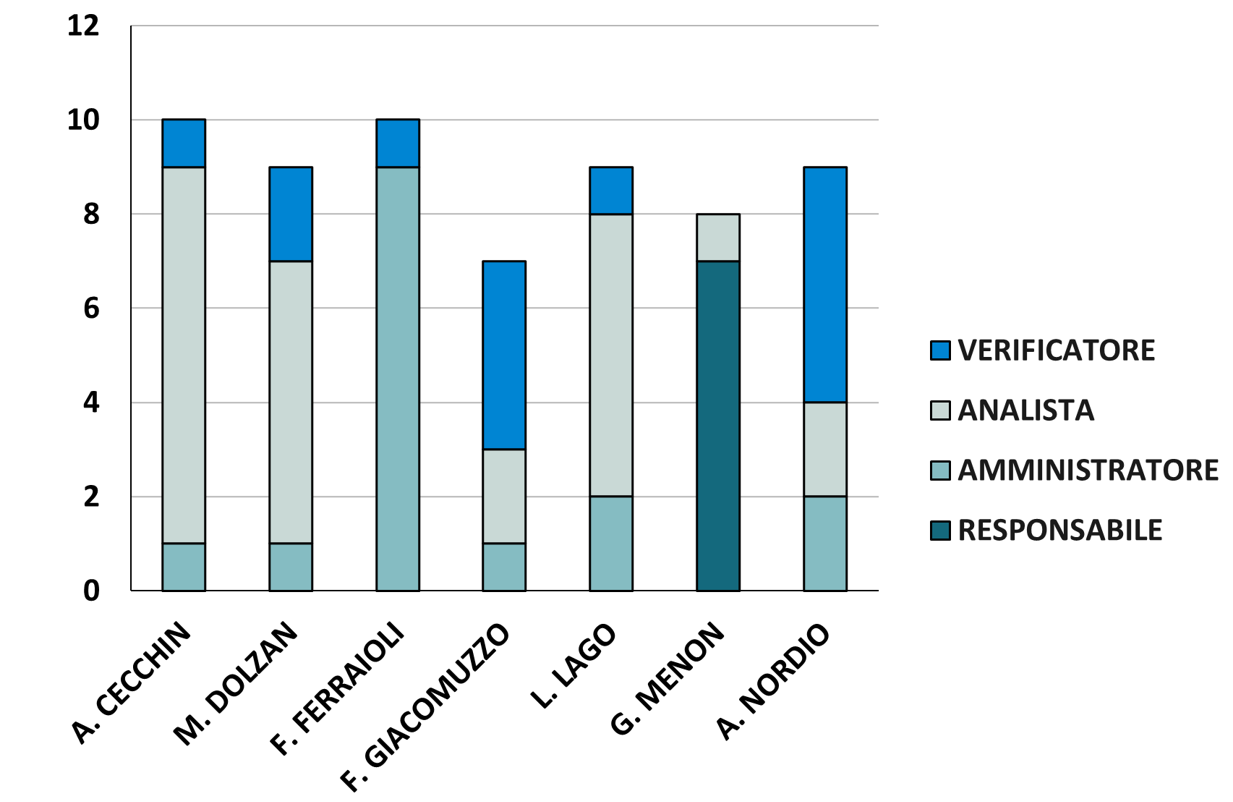
\includegraphics[width=0.75\textwidth]{cons1ruoli.png}
    \caption{Ruoli effettivi primo sprint}
    \label{fig:consuntivoorarioprimosprint}
\end{figure}

\newpage
\subsubsection{Consuntivo economico}
{
\setlength{\tabcolsep}{10pt}
\renewcommand{\arraystretch}{1.5}
\rowcolors{2}{oddrow}{evenrow}
\begin{table}[h]
    \centering
    \begin{tabularx}{\textwidth}{| l | l | l | X |}
        \hline
        \rowcolor{headerrow} \textbf{\textcolor{white}{Ruolo}} & \textbf{\textcolor{white}{Costo orario}} & \textbf{\textcolor{white}{Ore impiegate}} & \textbf{\textcolor{white}{Costo €}} \\
        \hline
        Responsabile & 30 & 7 & 210\\
        \hline
        Amministratore & 20 & 16 & 320\\
        \hline
        Progettista& 25 & 0  & 0\\
        \hline
        Analista & 25 & 25  & 625\\
        \hline
        Programmatore & 15 & 0  & 0\\
        \hline
        Verificatore & 15 & 14  & 210\\
        \hline
        \cellcolor{headerrow} \textbf{\textcolor{white}{Totale}} &  &  & \textbf{1365}\\
        \hline
        \cellcolor{headerrow} \textbf{\textcolor{white}{Rimanente}} &  &  & \textbf{11620}\\
        \hline
    \end{tabularx}
    \caption{Consuntivo economico primo sprint}
    \label{tab:consuntivocostiprimosprint}
\end{table}
}

\begin{figure}[h!]
    \centering
    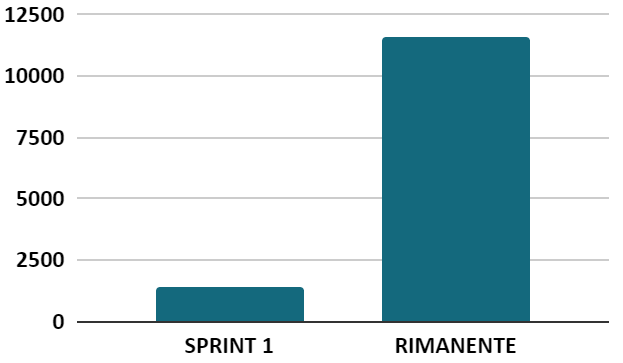
\includegraphics[width=0.8\textwidth]{cons1costo.png}
    \caption{Costo primo sprint e rimanente}
    \label{fig:consuntivocostoprimosprint}
\end{figure}

\newpage
\subsubsection{Analisi retrospettiva}
Analizzando le ore impiegate nel primo sprint, in relazione allo stato di avanzamento del progetto, il precedente periodo risulta essere positivo nel suo complesso. Da un'analisi collettiva è emersa una difficoltà da parte dei verificatori di svolgere il loro lavoro minimizzando quanto più il discostamento tra ore produttive e di orologio: questo a causa di una non sempre ottimale comunicazione interna al gruppo. Non è tuttavia ritenuta una questione di cui allarmarsi, in quanto l'elevato numero di ore impiegate nel ruolo di amministratore hanno portato alla realizzazione di \ccgloss{automazioni} a sostegno del lavoro di ogni membro. Con la possibilità di utilizzare l'ambiente di project management di \ccgloss{Jira} al massimo del suo potenziale nel prossimo sprint, si è sicuri di ottimizzare la distribuzione di task e diminuire il rapporto tra ore produttive e ore di orologio già citato.\\
Il massiccio impiego di analisti ha portato il documento di analisi dei requisiti (Analisi\_dei\_requisiti\_0.6) ad un ottimo punto, tanto che è stato fin da subito possibile esporre il lavoro fatto al proponente ricevendo feedback a riguardo.
\newpage

\subsection{Secondo sprint: 2023/11/20 - 2023/12/03}

\subsubsection{Consuntivo orario}
{
\setlength{\tabcolsep}{10pt}
\renewcommand{\arraystretch}{1.5}
\rowcolors{2}{oddrow}{evenrow}
\begin{table}[h!]
    \centering
    \begin{tabularx}{\textwidth}{| l | c | c | c | c | c | c | X |}
        \hline
        \rowcolor{headerrow} \textbf{\textcolor{white}{Membro}} & \textbf{\textcolor{white}{R.}} & \textbf{\textcolor{white}{Am.}} & \textbf{\textcolor{white}{Pj.}} & \textbf{\textcolor{white}{An.}} & \textbf{\textcolor{white}{Pg.}} & \textbf{\textcolor{white}{V.}} & \textbf{\textcolor{white}{Totale}} \\
        \hline
        Andrea Cecchin & - & 4 & 2 & - & 3 & - & \textbf{9} \\
        \hline
        Marco Dolzan & - & - & - & 1 & 6 & 3 & \textbf{10} \\
        \hline
        Francesco Ferraioli & - & - & 3 & 4 & - & 2 & \textbf{9} \\
        \hline  
        Francesco Giacomuzzo & 7 & - & - & - & - & 2 & \textbf{9} \\
        \hline
        Leonardo Lago & - & 4 & 2 & - & - & 3 & \textbf{9} \\
        \hline
        Giovanni Menon & - & - & 3 & 2 & 6 & - & \textbf{11} \\
        \hline
        Anna Nordio & - & 2 & - & 2 & 5 & - & \textbf{9} \\
        \hline
    \cellcolor{headerrow} \textbf{\textcolor{white}{Totale}} & \textbf{7} & \textbf{10} & \textbf{10} & \textbf{9} & \textbf{20} & \textbf{10} & \textbf{66} \\
        \hline
    \end{tabularx} 
    \caption{Consuntivo orario secondo sprint}
    \label{tab:consuntivoorariosecondosprint}
\end{table}
}

\begin{figure}[h!]
    \centering
    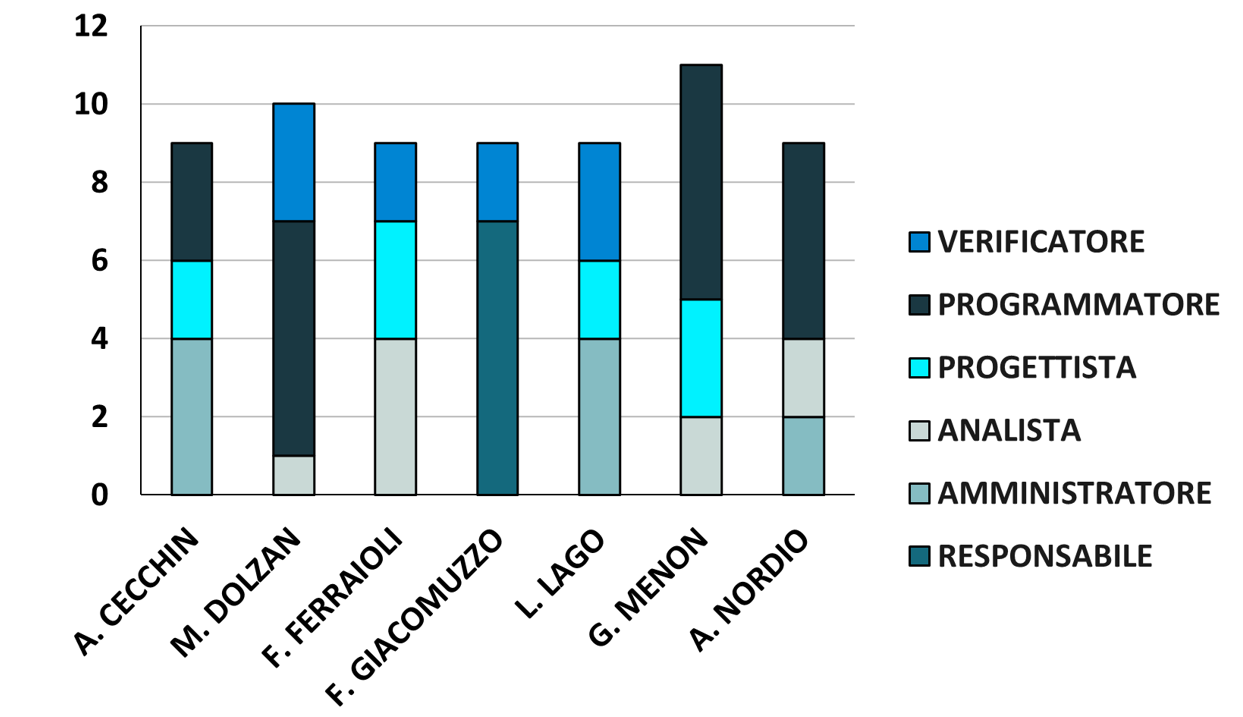
\includegraphics[width=0.8\textwidth]{cons2ruoli.png}
    \caption{Ruoli effettivi secondo sprint}
    \label{fig:consuntivoorariosecondosprint}
\end{figure}

\newpage
\subsubsection{Consuntivo economico}
{
\setlength{\tabcolsep}{10pt}
\renewcommand{\arraystretch}{1.5}
\rowcolors{2}{oddrow}{evenrow}
\begin{table}[h]
    \centering
    \begin{tabularx}{\textwidth}{| l | l | l | X |}
        \hline
        \rowcolor{headerrow} \textbf{\textcolor{white}{Ruolo}} & \textbf{\textcolor{white}{Costo orario}} & \textbf{\textcolor{white}{Ore impiegate}} & \textbf{\textcolor{white}{Costo €}} \\
        \hline
        Responsabile & 30 & 7 & 210\\
        \hline
        Amministratore & 20 & 10 & 200\\
        \hline
        Progettista& 25 & 10 & 250\\
        \hline
        Analista & 25 & 9 & 225\\
        \hline
        Programmatore & 15 & 20 & 300\\
        \hline
        Verificatore & 15 & 10 & 150\\
        \hline
        \cellcolor{headerrow} \textbf{\textcolor{white}{Totale}} &  &  & \textbf{1335}\\
        \hline
        \cellcolor{headerrow} \textbf{\textcolor{white}{Rimanente}} &  &  & \textbf{10285}\\
        \hline
    \end{tabularx}
    \caption{Consuntivo economico secondo sprint}
    \label{tab:consuntivocostisecondosprint}
\end{table}
}

\begin{figure}[h!]
    \centering
    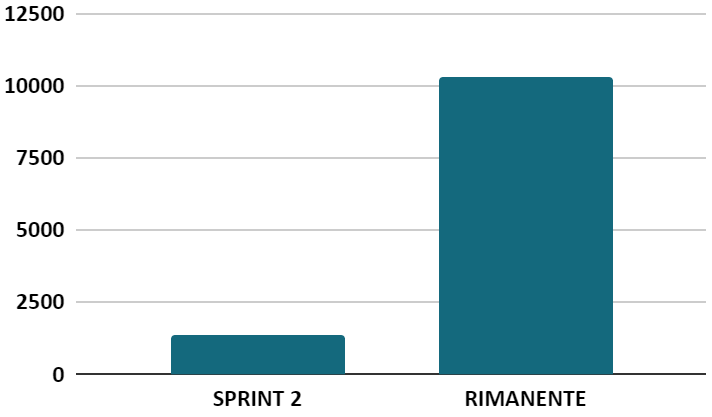
\includegraphics[width=0.8\textwidth]{cons2costo.png}
    \caption{Costo secondo sprint e rimanente}
    \label{fig:consuntivocostosecondosprint}
\end{figure}

\newpage
\subsubsection{Analisi retrospettiva}
Analizzando le ore utilizzate nel secondo sprint, in relazione allo stato di avanzamento del progetto, il precedente periodo risulta essere positivo nel suo complesso. In particolare l'elevato impegno orario nei ruoli di progettista e programmatore ha portato alla realizzazione di una PoC nel quale vengono impiegate le più rilevanti tecnologie trovate dal gruppo (langchain, Next.js, ChromaDB, Ollama e OpenAI). Il PoC fino a questo momento realizzato non può però definirsi completo in quanto manca l'integrazione di un database relazionale che permetta l'archivio dei documenti caricati nell'applicativo. Inoltre, è stata raggiunta una versione stabile del glossario (Glossario\_v0.14) contenente quindi tutti i termini e acronimi che potrebbero essere ambigui; tale versione non è però da considerarsi definitiva in quanto dovrà essere aggiornato con nuovi vocaboli che risultano poco chiari ad un lettore esterno. Il gruppo ha avanzato nella stesura del Way of Working (Norme\_di\_progetto\_v0.8); sono ancora assenti per contenuti le sezioni dedicate ai processi di verifica (§3.4),  validazione (§3.5) e gestione delle infrastrutture tecniche (§4.2). Dall'altro lato il piano di qualifica (Piano\_di\_qualifica\_v0.1) non ha ricevuto significativi avanzamenti. Il documento di analisi dei requisiti (Analisi\_dei\_requisiti\_v0.9) è stato aggiornato con i diagrammi UML e la stesura dei requisiti funzionali; mancano ancora le sezioni relative ai requisiti di qualità, vincolo e prestazionali. Questa assenza è dovuta ad una pianificazione debole che ha sottostimato il quantitativo orario dedicato alla programmazione del PoC e quindi ha assegnato un impegno temporale irrealistico all'attività di analisi. Da una riflessione collettiva è poi emerso una difficoltà nella suddivisione dei compiti, in issue assegnabili ad una singola persona, in particolare le issue risultano essere troppo "grandi" e generiche. Per questo motivo il gruppo ha deciso di aumentare il numero di issue create, diminuendo il carico di lavoro per ciascuna di esse. Un'altra problematica emersa riguarda la difficoltà di lavorare con i modelli scelti, in quanto richiedono, durante l'esecuzione, un elevato numero di risorse che i dispositivi di alcuni membri del gruppo non riescono a fornire. Ciò è stato risolto con l'utilizzo delle tecnologie messe a disposizione dall'azienda, in particolare un account OpenAI che permette l'utilizzo di modelli attraverso chiamate API riducendo al minimo la richiesta di risorse ai dispositivi.
\newpage

\subsection{Terzo sprint: 2023/11/04 - 2023/12/17}

\subsubsection{Consuntivo orario}
{
\setlength{\tabcolsep}{10pt}
\renewcommand{\arraystretch}{1.5}
\rowcolors{2}{oddrow}{evenrow}
\begin{table}[h!]
    \centering
    \begin{tabularx}{\textwidth}{| l | c | c | c | c | c | c | X |}
        \hline
        \rowcolor{headerrow} \textbf{\textcolor{white}{Membro}} & \textbf{\textcolor{white}{R.}} & \textbf{\textcolor{white}{Am.}} & \textbf{\textcolor{white}{Pj.}} & \textbf{\textcolor{white}{An.}} & \textbf{\textcolor{white}{Pg.}} & \textbf{\textcolor{white}{V.}} & \textbf{\textcolor{white}{Totale}} \\
        \hline
        Andrea Cecchin & - & 1 & - & - & 4 & 4 & \textbf{9} \\
        \hline
        Marco Dolzan & - & 4 & 2 & - & 3 & - & \textbf{9} \\
        \hline
        Francesco Ferraioli & - & - & - & 3 & 2 & 4 & \textbf{9} \\
        \hline  
        Francesco Giacomuzzo & - & - & 2 & 3 & - & 4 & \textbf{9} \\
        \hline
        Leonardo Lago & 6 & - & - & 2 & - & - & \textbf{8} \\
        \hline
        Giovanni Menon & - & 4 & - & 1 & 3 & - & \textbf{8} \\
        \hline
        Anna Nordio & - & - & 2 & 5 & 3 & - & \textbf{10} \\
        \hline
    \cellcolor{headerrow} \textbf{\textcolor{white}{Totale}} & \textbf{6} & \textbf{9} & \textbf{6} & \textbf{14} & \textbf{15} & \textbf{12} & \textbf{62} \\
        \hline
    \end{tabularx} 
    \caption{Consuntivo orario terzo sprint}
    \label{tab:consuntivoorarioterzosprint}
\end{table}
}

\begin{figure}[h!]
    \centering
    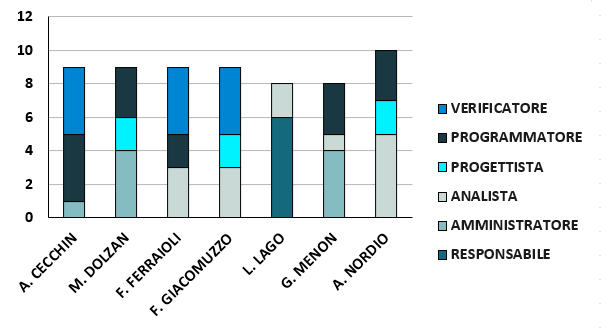
\includegraphics[width=0.8\textwidth]{cons3ruoli.png}
    \caption{Ruoli effettivi terzo sprint}
    \label{fig:consuntivoorarioterzosprint}
\end{figure}

\newpage
\subsubsection{Consuntivo economico}
{
\setlength{\tabcolsep}{10pt}
\renewcommand{\arraystretch}{1.5}
\rowcolors{2}{oddrow}{evenrow}
\begin{table}[h]
    \centering
    \begin{tabularx}{\textwidth}{| l | l | l | X |}
        \hline
        \rowcolor{headerrow} \textbf{\textcolor{white}{Ruolo}} & \textbf{\textcolor{white}{Costo orario}} & \textbf{\textcolor{white}{Ore impiegate}} & \textbf{\textcolor{white}{Costo €}} \\
        \hline
        Responsabile & 30 & 6 & 180\\
        \hline
        Amministratore & 20 & 9 & 180\\
        \hline
        Progettista& 25 & 6 & 150\\
        \hline
        Analista & 25 & 14 & 350\\
        \hline
        Programmatore & 15 & 15 & 225\\
        \hline
        Verificatore & 15 & 12 & 180\\
        \hline
        \cellcolor{headerrow} \textbf{\textcolor{white}{Totale}} &  &  & \textbf{1265}\\
        \hline
        \cellcolor{headerrow} \textbf{\textcolor{white}{Rimanente}} &  &  & \textbf{9020}\\
        \hline
    \end{tabularx}
    \caption{Consuntivo economico terzo sprint}
    \label{tab:consuntivocostiterzosprint}
\end{table}
}

\begin{figure}[h!]
    \centering
    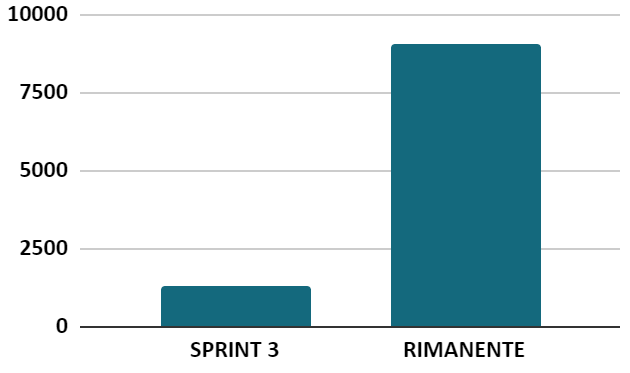
\includegraphics[width=0.8\textwidth]{cons3costo.png}
    \caption{Costo terzo sprint e rimanente}
    \label{fig:consuntivocostoterzpsprint}
\end{figure}

\newpage
\subsubsection{Analisi retrospettiva}
Analizzando le ore utilizzate nel terzo sprint, in relazione allo stato di avanzamento del progetto, il precedente periodo risulta essere abbastanza positivo nel suo complesso. In particolare l'elevato impegno orario nel ruolo di analista ha portato alla revisione dell'analisi dei requisiti.\\ Il PoC a questo momento ha subito numerosi miglioramenti sia per l'aggiunta di funzionalità, sia per il refactoring di alcune componenti, portandone lo stato complessivo a quasi completo.\\ Il Glossario non ha subito modifiche dallo sprint precedente, trovandosi tuttora ad una versione stabile (Glossario\_v0.14). È pianificato un aggiornamento di questo documento nei successivi sprint.\\ Il gruppo è avanzato nella stesura del Way of Working (Norme\_di\_progetto\_v0.11): sono tuttavia ancora assenti per contenuti le sezioni dedicate ai processi di verifica (§3.4) e gestione delle infrastrutture tecniche (§4.2).\\ Il Piano di qualifica (Piano\_di\_qualifica\_v0.3) ha subito degli avanzamenti ma risulta ancora incompleto.\\ Il documento di analisi dei requisiti (Analisi\_dei\_requisiti\_v0.12) ha ricevuto avanzamenti e revisioni agli Use Case, dovute al colloquio tenutosi con il Professor Cardin.\\ In generale diversi obiettivi inizialmente posti per essere conclusi in questo sprint risultano slittare e vedersi concludere indicativamente nello sprint successivo. Questo a causa anche delle ampie modifiche inattese di alcuni documenti, come l’analisi dei requisiti. Inoltre l’avvicinamento alla parte di programmazione a PoC già avviato di nuovi addetti ha causato qualche difficoltà. Si riscontra inoltre un leggero ristagno di verbali che rimango in stato di verificato ma non approvato per diverso tempo. Si segnala infine che gli incontri con il proponente, successivi all'approvazione del Proof of Concept, sono rallentati come da accordo tra le parti, preferendo contatti asincroni, e si nota un leggero ritardo nell'approvazione della modulistica da controfirmare.
\newpage


\subsection{Quarto sprint: 2023/11/18 - 2023/12/31}

\subsubsection{Consuntivo orario}
{
\setlength{\tabcolsep}{10pt}
\renewcommand{\arraystretch}{1.5}
\rowcolors{2}{oddrow}{evenrow}
\begin{table}[h!]
    \centering
    \begin{tabularx}{\textwidth}{| l | c | c | c | c | c | c | X |}
        \hline
        \rowcolor{headerrow} \textbf{\textcolor{white}{Membro}} & \textbf{\textcolor{white}{R.}} & \textbf{\textcolor{white}{Am.}} & \textbf{\textcolor{white}{Pj.}} & \textbf{\textcolor{white}{An.}} & \textbf{\textcolor{white}{Pg.}} & \textbf{\textcolor{white}{V.}} & \textbf{\textcolor{white}{Totale}} \\
        \hline
        Andrea Cecchin & - & -  & - & - & - & 6 & \textbf{6} \\
        \hline
        Marco Dolzan & - & - & - & - & 1 & 4 & \textbf{5} \\
        \hline
        Francesco Ferraioli & 4 & - & - & - & - & - & \textbf{4} \\
        \hline  
        Francesco Giacomuzzo & - & 3 & - & 2 & - & - & \textbf{5} \\
        \hline
        Leonardo Lago & - & - & - & 2 & 4 & - & \textbf{6} \\
        \hline
        Giovanni Menon & - & - & - & 3 & 1 & 4 & \textbf{8} \\
        \hline
        Anna Nordio & - & 2 & - & - & - & 4 & \textbf{6} \\
        \hline
    \cellcolor{headerrow} \textbf{\textcolor{white}{Totale}} & \textbf{4} & \textbf{5} & \textbf{0} & \textbf{7} & \textbf{6} & \textbf{18} & \textbf{40} \\
        \hline
    \end{tabularx} 
    \caption{Consuntivo orario quarto sprint}
    \label{tab:consuntivoorarioquartosprint}
\end{table}
}

\begin{figure}[h!]
    \centering
    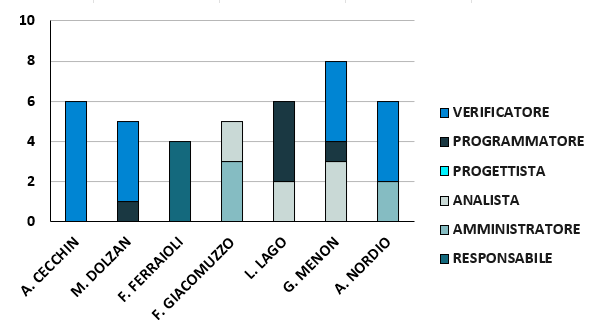
\includegraphics[width=0.8\textwidth]{cons4ruoli.png}
    \caption{Ruoli effettivi quarto sprint}
    \label{fig:consuntivoorarioquartosprint}
\end{figure}

\newpage
\subsubsection{Consuntivo economico}
{
\setlength{\tabcolsep}{10pt}
\renewcommand{\arraystretch}{1.5}
\rowcolors{2}{oddrow}{evenrow}
\begin{table}[h]
    \centering
    \begin{tabularx}{\textwidth}{| l | l | l | X |}
        \hline
        \rowcolor{headerrow} \textbf{\textcolor{white}{Ruolo}} & \textbf{\textcolor{white}{Costo orario}} & \textbf{\textcolor{white}{Ore impiegate}} & \textbf{\textcolor{white}{Costo €}} \\
        \hline
        Responsabile & 30 & 4 & 120\\
        \hline
        Amministratore & 20 & 5 & 100\\
        \hline
        Progettista & 25 & 0 & 0\\
        \hline
        Analista & 25 & 7 & 175\\
        \hline
        Programmatore & 15 & 6 & 90\\
        \hline
        Verificatore & 15 & 18 & 270\\
        \hline
        \cellcolor{headerrow} \textbf{\textcolor{white}{Totale}} &  &  & \textbf{755}\\
        \hline
        \cellcolor{headerrow} \textbf{\textcolor{white}{Rimanente}} &  &  & \textbf{8265}\\
        \hline
    \end{tabularx}
    \caption{Consuntivo economico quarto sprint}
    \label{tab:consuntivocostiquartosprint}
\end{table}
}

\begin{figure}[h!]
    \centering
    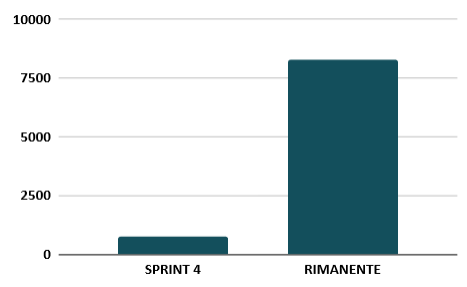
\includegraphics[width=0.8\textwidth]{cons4costo.png}
    \caption{Costo quarto sprint e rimanente}
    \label{fig:consuntivocostoquartopsprint}
\end{figure}

\newpage
\subsubsection{Analisi retrospettiva}
Analizzando le ore impiegate nel quarto sprint, in relazione allo stato di avanzamento del progetto, il periodo appena terminato risulta essere molto positivo.\\
L'elevato impiego orario nei ruoli di verificatore ha portato il Piano di qualifica ad una versione avanzata (Piano\_di\_qualifica\_v0.6), contenente tutte le metriche di prodotto e processo adottate, e un cruscotto con tutti i valori delle metriche individuate. L'aggiornamento dei grafici di questa sezione sarà coerentemente prevista nel prossimo periodo, così come ad ogni sprint, così da riportare i valori corretti. Risulta da aggiornare la sezione dei test (§2.4), con la definizione completa dei test di accettazione, l'introduzione del documento e quella della sezione Piano di qualità.\\
L'Analisi dei requisiti sembra giunta ad una versione definitiva (Analisi\_dei\_requisiti\_v0.18), con la stesura di tutte le sezioni previste, corrette a seguito del colloquio con il committente. Sono possibili piccoli aggiornamenti su di esso, in vista della revisione di avanzamento. Allo stesso modo, le Norme di progetto (Norme\_di\_progetto\_v0.13) sono avanzate con la stesura delle sezioni mancanti. È attualmente in corso la stesura, quasi completata, di un'ultima sezione (§3.4), dopo la quale il documento sarà ad una versione stabile, con futuri aggiornamenti di carattere integrativo.\\
Il Proof of Concept è, anche dopo questo sprint, ad una versione potenzialmente finale. Si è comunque deciso di proseguire nella sua programmazione, nel tentativo di migliorarlo in vista della revisione di avanzamento.
Non sono previsti particolari interventi sul Glossario, vicino all'approvazione finale.
\newpage
